\documentclass[a4paper]{report}

\usepackage[utf8]{inputenc}
\usepackage[T1]{fontenc}
\usepackage[american]{babel}
\usepackage{csquotes}
\usepackage[inline]{enumitem}
\usepackage{booktabs}
\usepackage[font=small,labelfont=bf]{caption}
\usepackage[group-separator={,}]{siunitx}
\usepackage{amsmath}
\usepackage{amssymb}
\usepackage{amsthm}
\usepackage[ruled,linesnumbered]{algorithm2e}
\usepackage{microtype}

\usepackage{listings}
\lstdefinestyle{mystyle}{
    basicstyle=\ttfamily\color{black!60},
    backgroundcolor=\color{black!5},
    commentstyle=\itshape\color{cyan},
    keywordstyle=\color{purple},
    keywordstyle=[2]\color{orange},
    identifierstyle=\color{black},
    numberstyle=\footnotesize\color{black},
    numbers=left,
    numbersep=4pt,
    columns=fixed,
}
\lstset{style=mystyle}
% Minimal support for WGSL, whatever is needed, based on C syntax
\lstdefinelanguage{WGSL}[ANSI]{C}%
    {morekeywords={let,var,fn},%
     morekeywords=[2]{u32,i32,bool},% Types
}

\usepackage{hyperref}
\hypersetup{
    colorlinks=true,
    linkcolor=blue,
    urlcolor=cyan,
    citecolor=teal,
    unicode=true,
}

\usepackage{tikz}
\usetikzlibrary{positioning}

\usepackage[style=numeric,urldate=ymd]{biblatex}
\addbibresource{bibliography.bib}

% Vertically centered vdots, taken from:
% https://tex.stackexchange.com/questions/112204/how-to-vertically-center-the-vdots-in-this-node
\makeatletter
\DeclareRobustCommand{\rvdots}{%
  \vbox{
    \baselineskip4\p@\lineskiplimit\z@
    \kern-\p@
    \hbox{.}\hbox{.}\hbox{.}
  }}
\makeatother

\theoremstyle{definition}
\newtheorem{definition}{Definition}

\title{
    {Accelerating Process Equivalence Energy Games using WebGPU}\\
    {\large Technische Universität Berlin}\\
}
\author{Gabriel Benediktus Vogel}

\begin{document}

\maketitle

%\begin{abstract}
%TODO Abstract
%\end{abstract}

\tableofcontents

\chapter{Introduction}
% Problem
In the field of process theory,
an often recurring question is that of
the behavioral similarity between processes in a transition system.
There are many different ways in which two processes can be considered
\emph{equivalent}.
In an important step towards grasping the range of equivalences,
\textcite{glabbeek1990spectrum} collected the most relevant definitions in the
so-called \emph{linear-time--branching-time spectrum}.
Being able to compute these equivalences is relevant for applications like
formal verification
or for gaining a better understanding of complex systems.

While algorithms for computing individual notions of equivalence
have long existed (e.g.~\cite{Blom2002}),
a process for deciding all equivalences of the spectrum at once
was only recently developed
by Bisping, Jansen and Nestmann~\cite{Bisping2022}.
This algorithm is subsequently refined by \textcite{bisping2023process}
where an \emph{energy game} is used for finding the equivalences.
This helps in bringing the runtime and memory usage of the algorithm down
to a more practical range,
but it is still very expensive to execute.
On larger inputs the implementation can easily run for the excess of several
minutes or even run out of memory.

% Contribution
This work aims to improve on that performance by utilizing the parallel
computing power of modern GPUs.
The idea is that large parts of the algorithm can be computed in parallel,
which, if successful, could result in a significant reduction in runtime.
To this end, the contribution of this thesis is the development
of \texttt{gpuequiv}%
\footnote{The code can be found at \url{https://github.com/Gobbel2000/gpuequiv}.
This document refers to version 1.0.0.},
a new, GPU-accelerated implementation
of the algorithm presented by \textcite{bisping2023process}.
It processes the most critical parts of the energy game in a highly
parallelized fashion
with the goal of making the spectroscopy algorithm faster and more scalable.
The same implementation can also be used more generally for solving energy
games.

For the task of interfacing with the GPU,
the WebGPU API is used.
WebGPU is a new web standard which currently is still in development,
with the goal of providing access to a system's GPU from web browsers.
By calling into WebGPU through the Rust library \texttt{wgpu} it is possible to
run the code both natively as well as from within a web site using WebAssembly.
This allows for very high platform-independence and portability.
Most of the code in \texttt{gpuequiv} is written in the
Rust programming language,
the GPU shaders are written in the WebGPU shading language WGSL\@.

\subsubsection{Related Work}

The broad structure for processing the energy game
is similar to a lot of other graph algorithms
by traversing the game graph in a breadth-first manner.
There is already a lot of research on running this category of graph
algorithms on a GPU~\cite{Merrill2015,Busato2018,Hijma2023}.
Similar projects exist in the context of transition systems,
for example a parallel algorithm for computing bisimilarity
by \textcite{Martens2023}
or a tool for detecting deadlocks in a transition system
by \textcite{Wijs2023},
both running on a GPU\@.
However, none of them give information
regarding the entire equivalence spectrum.

\subsubsection{Structure}

The following two chapters will introduce some of the concepts required to
fully understand the implementation choices behind \texttt{gpuequiv}.
Chapter~\ref{ch:processes} starts with defining processes and equivalences,
then continues to introducing the details of
the spectroscopy algorithm (\ref{sec:spectroscopy})
and of the energy game at its core (\ref{sec:energy_games}).
Chapter~\ref{ch:gpu} focuses on another important topic for this work:
GPU programming.
This includes details on the technology stack used
and the choice of WebGPU among other GPU frameworks,
followed by a short overview on what it means
to program for a GPU (\ref{sec:gpu_model}).

The actual GPU-based implementation of the spectroscopy algorithm is explained
in Chapter~\ref{ch:implementation}.
It begins with a more high-level look at how parallelization was achieved
(\ref{sec:parallelization}),
but also includes more technical details about the data layouts
used to efficiently handle the data (\ref{sec:data}).
Finally, in Chapter~\ref{ch:benchmarks} we will evaluate the performance
gained by parallelization with a series of benchmarks, which were
conducted both on \texttt{gpuequiv} as well as on the original implementation
by \textcite{bisping2023process}.


\chapter{Processes and Equivalences}
With the goal of presenting the algorithm for finding equivalences between
processes,
this chapter will introduce the theoretical concepts that this work is based on.
First and foremost this includes an explanation and definition
of the models we use to represent processes.
Further, we will explore different ways to compare two processes and how that
leads us to the equivalence spectrum~\cite{glabbeek1990spectrum}.
Finally, we will outline the spectroscopy algorithm,
which gives us a multifaceted view of the relation of two processes
by testing all of those equivalences at once~\cite{bisping2023process}.


\section{Modeling Processes}

We represent processes in a directed graph.
The outgoing edges of a node are the possible steps it can perform next.
Each edge is labelled with a specific action that occurs when taking that step.
After performing an action,
the process enters a new state represented by another node,
which is itself a process with its set of actions.
This forms a sort of state machine that at every step
moves to some other state by performing one of the currently available actions.
The series of actions being chosen
constitutes the observable behavior of the machine,
while its current state defines what actions it can do next.
Such a structure is called a \emph{Labeled transition system}
or \emph{LTS} for short~\cite{reactive_systems}.
Figure~\ref{fig:example_lts} gives an example for what the graph of an LTS might
look like.

\begin{definition}[Labeled Transition System~\cite{reactive_systems}]
    A labeled transition system is a triple
    $(\mathsf{Proc}, \mathsf{Act}, {\rightarrow})$
    where:

    \begin{itemize}
        \item $\mathsf{Proc}$ is the set of states or processes,
        \item $\mathsf{Act}$ is a set of actions,
        \item ${\rightarrow} \subseteq \mathsf{Proc} \times \mathsf{Act} \times \mathsf{Proc}$
            is the transition relation.
            We also write
            $p \xrightarrow{\alpha} p'$ for $(p, \alpha, p') \in {\rightarrow}$,
            meaning we can transition from state $p$ to $p'$
            using the action $\alpha$.
    \end{itemize}
\end{definition}

\begin{figure}[tb]
\begin{center}
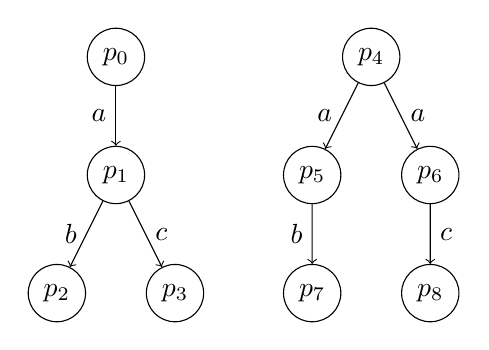
\begin{tikzpicture}[p/.style={circle,draw},->]
    \node[p] (0) {$p_0$}
        child {node[p] {$p_1$}
            child {node[p] {$p_2$} edge from parent node[left] {$b$}}
            child {node[p] {$p_3$} edge from parent node[right] {$c$}}
            edge from parent node[left] {$a$}
        };
    \node[p] (4) [right=25mm of 0] {$p_4$}
        child {node[p] {$p_5$}
            child {node[p] {$p_7$} edge from parent node[left] {$b$}}
            edge from parent node[left] {$a$}
        }
        child {node[p] {$p_6$}
            child {node[p] {$p_8$} edge from parent node[right] {$c$}}
            edge from parent node[right] {$a$}
        };
\end{tikzpicture}
\end{center}
\caption{An example for an LTS\@. In this case,
    $\mathsf{Proc} = \{p_0, p_1, \ldots, p_8\}$ and
    $\mathsf{Act} = \{a, b, c\}$.
}%
\label{fig:example_lts}
\end{figure}


\section{Equivalences Between Processes}

One of the most important questions that arises in the context of transition
systems is whether two processes show the same behavior.
This is a difficult question
because there are many different ways to define
what \emph{equivalent behavior} means.
This section will present two important definitions: Trace equivalence and
Bisimilarity.

\subsubsection{Trace Equivalence}

A simple way to qualify the behavior of a process is to look at the possible
strings of actions (traces) it can perform.
This is particularly apparent when viewing an LTS as a sort of automaton.
A sequence of actions $\alpha_1, \ldots, \alpha_k \in \mathsf{Act}^*$
is a trace of a process $p$ if
$p \xrightarrow{\alpha_1} p_1 \xrightarrow{\alpha_2} p_2
\ldots p_{k-1} \xrightarrow{\alpha_k} p_k$.
The function $\mathit{Traces}(p)$ produces the set of all traces
for a process $p$.
We now call two processes $p$ and $q$ \emph{trace-equivalent}
if $\mathit{Traces}(p) = \mathit{Traces}(q)$~\cite{reactive_systems}.

For example, in Figure~\ref{fig:example_lts} the traces of $p_0$ are
$\mathit{Traces}(p_0) = \{a, ab, ac\}$.
The process $p_4$ can produce exactly the same traces,
so $p_0$ and $p_4$ are trace-equivalent.
However it is not difficult to see some difference in the graphs of both
processes that this comparison seems to ignore.
Indeed, trace equivalence is one of the weakest equivalence notions,
meaning it more easily equates processes.
An even weaker equivalence would be \emph{enabledness},
which already equates two processes
if they have the same set of enabled actions,
given as
$\mathcal{I}(p) \colonequals \{\alpha \in \mathsf{Act} \mid
    {\exists p' \in \mathsf{Proc}}\,.\,p \xrightarrow{\alpha} p'\}$
for a process $p$.

Trace-equivalence, as well as many other equivalences,
can also be seen directionally.
If one only cares about whether all traces of $p$ are also traces in $q$ and
not the other way around---meaning
$\mathit{Traces}(p) \subseteq \mathit{Traces}(q)$---the result is a
preorder instead of an equivalence relation where $p$ is preordered by $q$
if the condition holds.


\subsubsection{Bisimilarity}

\emph{Bisimilarity} is special because it is the strongest of the behavioral
equivalences.
It requires two processes to provide the same set of actions not only initially,
but also after every time both processes have been advanced
by the same chain of actions.
It is defined as follows:

\begin{definition}[Bisimulation~\cite{reactive_systems}]\label{def:bisimulation}
    Processes $p, q \in \mathsf{Proc}$ are bisimilar, written $p \sim q$,
    if and only if there exists a relation
    $\mathcal{R} \subseteq \mathsf{Proc} \times \mathsf{Proc}$
    with $p\, \mathcal{R}\, q$ and for every $s_1\, \mathcal{R}\, s_2$ and
    $\alpha \in \mathsf{Act}$:
    \begin{itemize}
        \item if $s_1 \xrightarrow{\alpha} s_1'$, then there is a transition
            $s_2 \xrightarrow{\alpha} s_2'$ such that $s_1'\, \mathcal{R}\, s_2'$,
        \item if $s_2 \xrightarrow{\alpha} s_2'$, then there is a transition
            $s_1 \xrightarrow{\alpha} s_1'$ such that $s_1'\, \mathcal{R}\, s_2'$.
    \end{itemize}
    A relation $\mathcal{R}$ satisfying these conditions is called a
    \emph{bisimulation}.
\end{definition}

This does not hold for our example in Figure~\ref{fig:example_lts}.
If we were trying to construct a bisimulation relation with
$p_0\, \mathcal{R}\, p_4$,
that would require $p_1\, \mathcal{R}\, p_5$
because $p_0 \xrightarrow{a} p_1$ and $p_4 \xrightarrow{a} p_5$.
But $p_1$ has a $c$-transition to $p_3$ which $p_5$ cannot simulate,
thus there is no bisimulation that relates $p_0$ and $p_4$.


\subsection{Hennessy--Milner Logic}

A very useful tool when discussing process equivalences is the
Hennessy--Milner logic (or HML),
which is a modal logic that can be used to formalize various
properties of a process.
A process satisfies a HML-formula if it observes
the property specified by the formula,
otherwise it does not satisfy it.
We adopt the syntax from~\cite{bisping2023process},
which is slightly different although functionally equivalent to the definition
in~\cite{reactive_systems}.
This is relevant because we will later require precise control over the
structure of HML-formulas.

\begin{definition}[%
    Hennessy--Milner logic~\cite{bisping2023process,reactive_systems}]%
    \label{def:hml}
    The set $\mathcal{M}$ of HML-formulas over a set of actions $\mathsf{Act}$
    is constructed by the following grammar:
    \begin{align*}
        \varphi \coloncolonequals\ &\langle \alpha \rangle \varphi,
            \qquad \alpha \in \mathsf{Act} \\
            \mid \quad &\bigwedge \{\psi, \psi, \ldots\} \\
        \psi \coloncolonequals\ &\neg \varphi \mid \varphi
    \end{align*}
    The semantics $\llbracket \varphi \rrbracket$ of a formula
    $\varphi$ in a given LTS
    $(\mathsf{Proc}, \mathsf{Act}, {\rightarrow})$ denotes the set of processes in
    $\mathsf{Proc}$ that satisfy $\varphi$.
    It is recursively defined as:
    \begin{align*}
        \llbracket \langle \alpha \rangle \varphi \rrbracket &\colonequals
            \{p \in \mathsf{Proc} \mid
              \exists p' \in \llbracket \varphi \rrbracket\,.\,
              p \xrightarrow{\alpha} p'
            \} \\
        \llbracket \neg \varphi \rrbracket &\colonequals
            \mathsf{Proc} \setminus \llbracket \varphi \rrbracket \\
        \llbracket \bigwedge_{i \in I} \psi_i \rrbracket &\colonequals
            \bigcap_{i \in I} \llbracket \psi_i \rrbracket
    \end{align*}
    We use $\llbracket \neg \varphi \rrbracket$,
    but $\neg \varphi$ is not a member of $\mathcal{M}$:
    negated formulas can only occur inside a conjunction.
    The recursion in the above definition can be terminated using the empty
    conjunction $\top \colonequals \bigwedge \{\}$
    which itself always evaluates to true:
    $\llbracket \top \rrbracket = \mathsf{Proc}$.

    For $p \in \mathsf{Proc},\, \varphi \in \mathcal{M}$
    we write $p \models \varphi$ if, and only if,
    $p \in \llbracket \varphi \rrbracket$,
    meaning $p$ satisfies the formula $\varphi$.
\end{definition}

To give a few examples,
both $p_0$ and $p_4$ of Figure~\ref{fig:example_lts} satisfy the HML-formula
$\langle a \rangle \langle b \rangle \top$,
which requires an $a$-transition followed by a $b$-transition,
thus encoding the trace $ab$.
However the formula
$\varphi = \langle a \rangle \bigwedge \{
    \langle b \rangle \top, \langle c \rangle \top \}$
is only satisfied by $p_0$, not by $p_4$,
since it requires an $a$-transition
after which both actions $b$ and $c$ should be possible.
$p_4$ does have two $a$-transitions,
but neither $p_5$ nor $p_6$ offers both $b$ and $c$.
Therefore, $\varphi$ is a \emph{distinguishing formula} for $p_0$ and $p_4$,
since it points out a difference in their behavior.


\subsection{The Equivalence Spectrum}

A number of behavioral equivalences have been collected and ordered
in the \emph{linear-time--branching-time spectrum}
by \textcite{glabbeek1990spectrum}.
By examining subsets of HML-formulas we can achieve a general definition
for all equivalences,
which is a crucial step towards our goal of testing all of them at once.

Each notion of equivalence is characterized by a subset of HML-formulas
$\mathcal{O} \subseteq \mathcal{M}$.
If the subset includes a distinguishing formula for two processes $p$ and $q$,
$\exists \varphi \in \mathcal{O}\,.\,
    p \models \varphi \wedge q \not\models \varphi$,
that equivalence does not hold, it is refuted by $\varphi$.
If there is no such formula,
$p$ is preordered by $q$ with respect to the chosen equivalence.
Only if $q$ is also preordered by $p$,
meaning there is also no distinguishing formula $\varphi' \in \mathcal{O}$
with $q \models \varphi'$ and $p \not\models \varphi'$,
can we call $p$ and $q$ equivalent with respect to the chosen set of formulas.

\textcite{bisping2023process} represents these subsets of $\mathcal{M}$
by assigning a 6-dimensional \enquote{expressiveness price} to each formula
and construcing the subsets by including all formulas below a maximum price.
Without going further into the exact definition of the prices,
all equivalences, along with their price vector representing a subset of
HML-formulas are listed in Table~\ref{tab:spectrum}.

\begin{table}[htpb]
    \centering
    \caption{Equivalences of the linear-time--branching-time spectrum and the
        maximum expressiveness a HML-formula may have to refute this
        equivalence~\cite{bisping2023process}.}%
    \label{tab:spectrum}
    \begin{tabular}{l l}
        \toprule
        Equivalence &Price \\
        \midrule
        Bisimulation &$(\infty, \infty, \infty, \infty, \infty, \infty)$ \\
        2-nested Simulation &$(\infty, \infty, \infty, \infty, \infty, 1)$ \\
        Ready Simulation &$(\infty, \infty, \infty, \infty, 1, 1)$ \\
        Readiness Traces &$(\infty, \infty, \infty, 1, 1, 1)$ \\
        Possible Futures &$(\infty, 2, \infty, \infty, \infty, 1)$ \\
        Simulation &$(\infty, \infty, \infty, \infty, 0, 0)$ \\
        Failure Traces &$(\infty, \infty, \infty, 0, 1, 1)$ \\
        Readiness &$(\infty, 2, 1, 1, 1, 1)$ \\
        Revivals &$(\infty, 2, 1, 0, 1, 1)$ \\
        Impossible Futures &$(\infty, 2, 0, 0, \infty, 1)$ \\
        Failures &$(\infty, 2, 0, 0, 1, 1)$ \\
        Traces &$(\infty, 1, 0, 0, 0, 0)$ \\
        Enabledness &$(1, 1, 0, 0, 0, 0)$ \\
        \bottomrule
    \end{tabular}
\end{table}

The strongest equivalence, bisimulation, puts no restrictions on the price of
distinguishing formulas: all components are set to $\infty$.
This property is famously characterized by the Hennessy--Milner-theorem,
stating that two processes are bisimilar if, and only if,
they satisfy exactly the same HML-formulas~\cite{reactive_systems}.


\section{Energy Games}\label{sec:energy_games}

The question of finding equivalences can now be reformulated to ask instead
about the costs required to distinguish two processes.
Once that is known, the set of satisfied equivalences can be derived from
Table~\ref{tab:spectrum}.
These costs are computed with the help of an \emph{energy game},
which is an extension over the classic \emph{reachability game}.

In a reachability game,
the goal of the attacker player is to reach a predefined set of target positions,
while the defender tries to prevent it.
The energy game simply adds the restriction that the attacker must also start
out with a sufficient \emph{energy budget},
which is decreased at every step.
In order to support multiple, independent cost factors,
these energies can be multidimensional:

\begin{definition}[Energies~\cite{bisping2023process,brihaye2023multi}]%
    \label{def:energies}
    The set of $N$-dimensional energies is given as
    \[\mathbf{En}_N \colonequals {(\mathbb{N} \cup \{ \infty \})}^N.\]
    Energy tuples are compared component-wise, which creates a partial order:
    \[(e_1, \ldots, e_N) \leq (f_1, \ldots, f_N) \Leftrightarrow e_i \leq f_i
    \quad \text{for all } i \in [N].\]
    The supremum between two energy tuples is defined as usual:
    \[\sup((e_1, \ldots, e_N), (f_1, \ldots, f_N)) \colonequals
        (\max(e_1, f_1), \ldots, \max(e_N, f_N)).\]
    The upward closure $\upclosed E$ for a set of energies
    $E \subseteq \mathbf{En}$ contains all energies that are greater or equal
    to an element in $E$:
    \[\upclosed E \colonequals
        \{e \in \mathbf{En} \mid \exists e' \in E\,.\,e \geq e'\}\]
    Conversely, we can reduce an energy set $E \subseteq \mathbf{En}$
    to its minimal elements:
    \[\mathrm{Min} (E) \colonequals
        \{e \in E \mid \nexists e' \in E\,.\,e' \leq e \wedge e' \ne e\}\]
\end{definition}

We will construct the energy game in such a way that the attacker essentially
aims to point out a distinction between two processes,
while the energy budget required by the attacker could be seen as the
expressiveness cost of a formula encoding that distinction.
The prices in Table~\ref{tab:spectrum} are elements of $\mathbf{En}_6$ and
bring us back from energies to equivalences.

When discussing the energy game it will be convenient to consider
upwards-closed energy sets $\upclosed E$,
but when the energies are based on the natural numbers,
these sets are obviously infinite in size.
In practice we only store minimized energy sets $\mathrm{Min}(E)$.
Because all energies in a minimized set are incomparable to each other,
they form an antichain.
Such an antichain, representing a larger upwards-closed set,
is also referred to as a \emph{Pareto frontier}~\cite{brihaye2023multi}.

In the regular energy game as presented by \textcite{brihaye2023multi},
energies are simply reduced by subtracting another vector of natural numbers.
However for the purpose of the spectroscopy algorithm,
we require a special update function that includes $\minupd$-updates.
It is important to note that with this definition energies are only ever
\emph{decreased} by an update:
$\mathsf{upd}(e, u) \leq e$ for all $u \in \mathbf{Up}$.
The following definitions closely follow \textcite{bisping2023process},
who first proposed the usage of energy games for equivalence analysis.

\begin{definition}[Energy Updates~\cite{bisping2023process}]\label{def:update}
    The set of $N$-dimensional energy updates $\mathbf{Up}_N$ contains
    $N$-tuples $(u_1, \ldots, u_N) \in \mathbf{Up}_N$ where each update $u_k, k
    \in [N]$ is
    either
    \begin{itemize}
        \item $u_k \in \{-1, 0\}$, or
        \item $u_k = \minupd_D$ where $D \subseteq [N]$ and $k \in D$.
    \end{itemize}

    The partial function
    $\mathsf{upd}_N: (\mathbf{En}_N, \mathbf{Up}_N) \rightharpoonup \mathbf{En}_N$
    applies an update to an energy tuple.
    The $k$-th component is given as:
    \begin{equation*}
        \mathsf{upd}_N{(e, u)}_k =
        \begin{cases}
            e_k + u_k,\quad &\text{if } u_k \in \{-1, 0\} \text{ and } e_k \geq 1, \\
            \min_{d \in D}{e_d},\quad &\text{if } u_k = \minupd_D.
        \end{cases}
    \end{equation*}
\end{definition}

\begin{definition}[Energy Games~\cite{bisping2023process}]\label{def:energy_game}
    We define an $N$-dimensional energy game as
    $(G, G_a, G_d, E, w, g_0, e_0)$, where
    \begin{itemize}
        \item $G$ is a set of game positions.
        \item $G_a$ and $G_d$ are the sets of attacker and defender positions
            respectively.
            $G = G_a \cup G_d$ and $G_a \cap G_d = \emptyset$.
        \item $E \subseteq (G \times G)$ is the edge relation. $(G, E)$
            together form a directed game graph.
        \item $w: E \rightarrow \mathbf{Up}_N$ is a weight function, assigning an
            energy update to each edge.
        \item $g_0 \in G$ is the start position of the game.
        \item $e_0 \in \mathbf{En}_N$ is the starting energy budget of the attacker.
    \end{itemize}

    The function $\mathrm{Succ}: G \rightarrow 2^G$ gives the successors in the
    graph for a position.
    For each $g \in G$, $\mathrm{Succ}(g) = \{g' \in G \mid (g, g') \in E\}$.
    Similarly, $\mathrm{Pred}(g) = \{g' \in G \mid (g', g) \in E\}$ yields a
    position's predecessors.
\end{definition}

\begin{definition}[Plays and Costs~\cite{bisping2023process}]
    A \emph{play} $\rho$ on a given game is a sequence of positions:
    $\rho = g_0g_1 \ldots g_n$ where at each step
    $g_i \in G$ and $(g_i, g_{i+1}) \in E$.

    The energy level at step $i$ in the play $\rho$, $\mathsf{EL}_\rho(i)$,
    is initially $\mathsf{EL}_\rho(0) \colonequals e_0$.
    After each step the energy level is updated:
    $\mathsf{EL}_\rho(i + 1) \colonequals
        \mathsf{upd}(\mathsf{EL}_\rho(i), w(g_i, g_{i+1}))$.
    A step from $g_i$ to $g_{i+1}$ is not allowed
    if there is not enough energy left for it,
    in which case $\mathsf{upd}(\mathsf{EL}_\rho(i), w(g_i, g_{i+1}))$ is undefined.

    If a play cannot be further extended,
    that is either the energy was depleted or
    $\mathrm{Succ}(g_n) = \emptyset$,
    that play is won by the player who is not stuck:
    if $g_n \in G_a$, the defender wins, if $g_n \in G_d$, the attacker wins.
    Infinite plays are won by the defender.
\end{definition}

The problem we want to investigate now is
what the minimum required energies are
in order for the attacker to win the game,
regardless of the defender's decisions.
For a starting point $g_0 \in G$ we denote this set of winning budgets as
$W(g_0) \subseteq \mathbf{En}$.
If we find one energy tuple $e \in W(g_0)$ that is sufficient to win the game,
we know that all greater energies $e' \geq e$ must also lie in $W(g_0)$.
Therefore, $W(g_0)$ is an upwards-closed set and we will often just consider
its minimal elements $\mathrm{Min}(W(g_0))$.
Exactly this task of finding the minimal winning budgets in an energy game
is at the center of what this work tackles with the help of GPU-acceleration,
and will be further elaborated in Chapter~\ref{ch:implementation}.


\section{Spectroscopy Algorithm}\label{sec:spectroscopy}

The entire spectroscopy algorithm can now be outlined by
first generating an energy game for a given LTS,
and then computing the winning budgets for that particular game.
These winning budgets then represent the costs required to distinguish a
process pair,
which can be translated into some of the common equivalence notions.
The part that still remains is how to construct the energy game
so it actually serves to inform us about distinctions between processes.
Here it will suffice to briefly recapitulate the rules that are used to
construct the game graph.
A more extensive justification for them is provided in~\cite{bisping2023process}.

The game graph for an transition system
$(\mathsf{Proc}, \mathsf{Act}, {\rightarrow})$
is constructed around three types of game positions:

\begin{itemize}
    \item Attacker positions ${(p, Q)}_a \in G_a$
    \item Attacker clause positions ${(p, q)}_a^{\scriptscriptstyle\land} \in G_a$
    \item Defender positions ${(p, Q, Q_*)}_d \in G_d$
\end{itemize}

$p, q \in \mathsf{Proc}$ and $Q, Q_* \subseteq \mathsf{Proc}$.
The graph is induced by the following rules,
which define the edge relation $E$, as well as the update weights $w$.
The transition over sets $Q \xrightarrow{\alpha} Q'$
is defined as
$Q' = \{q' \in \mathsf{Proc} \mid
    \exists q \in Q\,.\,q \xrightarrow{\alpha} q'\}$.


\begin{table}[h!]
\centering

\begin{tabular}{l l l l}
    \toprule
    Position &Update &Next Position &Conditions \\
    \midrule
    ${(p, Q)}_a$ &$(-1, 0, 0, 0, 0, 0)$ &${(p', Q')}_a$
        &$p \xrightarrow{\alpha} p', Q \xrightarrow{\alpha} Q'$, \\
      &&&$p' \notin Q', Q \neq \emptyset$ \\
    ${(p, Q)}_a$ &$(0, -1, 0, 0, 0, 0)$ &${(p, Q \setminus Q_*, Q_*)}_d$
        &$Q_* \subsetneq Q, Q_* \in \mathcal{Q}$ \\
    ${(p, Q, Q_*)}_d$ &$(\minupd_{\{1, 3\}}, 0, 0, 0, 0, 0)$ &${(p, Q_*)}_a$
        &$Q_* \neq \emptyset$ \\
    ${(p, Q, Q_*)}_d$ &$(0, 0, 0, \minupd_{\{3, 4\}}, 0, 0)$
        &${(p, q)}_a^{\scriptscriptstyle\land}$
        &for $q \in Q$ \\
    ${(p, q)}_a^{\scriptscriptstyle\land}$
        &$(\minupd_{\{1, 4\}}, 0, 0, 0, 0, 0)$
        &${(p, \{q\})}_a$ \\
    ${(p, q)}_a^{\scriptscriptstyle\land}$
        &$(\minupd_{\{1, 5\}}, 0, 0, 0, 0, -1)$
        &${(q, \{p\})}_a$ \\
    \bottomrule
\end{tabular}
\end{table}

These rules already contain some optimizations that reduce the final game graph
size without affecting the results.
Defender positions are limited to cases
${(p, Q \setminus Q_*, Q_*)}_d$ with
$Q_* \in \mathcal{Q} \colonequals
\big\{\emptyset,
    \{q \in Q \mid \mathcal{I}(p) \subseteq \mathcal{I}(q)\},
    \{q \in Q \mid {\mathcal{I}(p) \supseteq \mathcal{I}(q)}\},
    \{q \in Q \mid \mathcal{I}(p) =         \mathcal{I}(q)\}
\big\}$,
where $\mathcal{I}(p)$ is the set of enabled actions of $p$.
This restriction to at most four different partitions
based on the enabled actions is called the
\enquote{clever spectroscopy game} in~\cite{bisping2023process}.
Generating defender positions ${(p, \emptyset, Q)}_d$ from ${(p, Q)}_a$
is also not required,
because their only successor is ${(p, Q)}_a$ again.
That loop does not influence the final winning budgets,
therefore the partitions $Q_*$ are limited to strict subsets of $Q$.

The meaning behind an attacker position ${(p, Q)}_a$ is roughly
that the attacker wants to distinguish $p$ from all processes in $Q$.
The game graph is typically seeded with one or more attacker positions
in the form ${(p, \{q\})}_a$.
Starting from there the graph is then recursively built up
using the rules above.
Finally, the winning budgets for a starting position,
$W({(p, \{q\})}_a)$,
are exactly the costs required to distinguish $p$ and $q$.

Subsequently, attack positions ${(p, Q)}_a$ with $p \in Q$ can be left out
since it is impossible to distinguish $p$ from itself.
This means the attacker can never win starting from such a position,
thus not contributing any winning budgets to other positions either.
If an attacker position ${(p, Q)}_a$ contains the empty set $Q = \emptyset$,
the attacker can win straight away by transitioning to
${(p, \emptyset, \emptyset)}_d$, which has no further successors.
No better costs can be achieved by considering further observations from $p$
and transitioning to any position ${(p', \emptyset)}_a$.


\chapter{GPU Compute Programming}\label{ch:gpu}
The core contribution of this work is a GPU-accelerated implementation of the
spectroscopy algorithm presented in~\cite{bisping2023process},
using the new WebGPU standard.
This chapter will give an overview on why WebGPU was chosen and how that
standard came to be among other GPU compute frameworks.
Further we will discuss the GPU programming model,
how its massively parallelized architecture can be utilized
and which challenges it raises.

\section{WebGPU and the State of GPU Compute}

As their name suggests, Graphics Processing Units (GPUs) were initially built
to improve graphical processing capabilities of computer systems,
serving as \emph{graphics accelerators}.
At first they included mostly fixed-function hardware to run the usual
rendering pipeline.
This required the same calculations to be performed for every object to
be rendered and every pixel on the screen,
which was solved by running as much as possible in parallel in order to produce
fluent frame rates.
These graphics accelerators enabled real-time rendering performance far beyond
what is possible on a general-purpose CPU,
which is why their development was largely driven
by the gaming industry~\cite{Patterson2016}.

But already early on people recognized the potential of using the parallel
GPU architecture not just for graphics rendering,
but for any kind of general-purpose computing that requires performing the same
instructions on a large amount of data.
GPUs gradually moved away from the fixed-function design and gained more
fine-grained programmability.
Along with that, specific programming environments were
developed to provide an easier interface for writing GPU compute programs.
Nvidia has long dominated the market by investing early in its
proprietary CUDA platform which supports Nvidia hardware only.
AMD has more recently been working on ROCm for their own GPUs.
OpenCL was meant to be a more portable alternative.

In another area WebGL was developed to bring GPU support into web browsers.
This was mainly intended for simpler graphics applications and is based on the
long-standing OpenGL graphics API\@.
Because of that, WebGL never really supported general-purpose compute programs.
Any efforts to improve this situation were abandoned%
\footnote{\url{https://registry.khronos.org/webgl/specs/latest/2.0-compute}}
in favor of a new browser API\@: WebGPU\@.
Instead of OpenGL, WebGPU is based on more advanced graphics APIs
that expose modern GPU features:
Vulkan for Linux and Windows, DX12 for Windows and Metal for Apple.
General-purpose compute is one of the express features for WebGPU,
thus providing a GPU programming API that is not only fully
platform-independent, but will even be able to run in any web browser.
However, as of the time of writing, the WebGPU specification is still in
development and full browser support is not yet available%
\footnote{\url{https://github.com/gpuweb/gpuweb/wiki/Implementation-Status}}.

For the GPU code, this work uses \texttt{wgpu}, an implementation of the WebGPU
standard written in the Rust programming language.
Applications using \texttt{wgpu} can both run natively, directly interfacing with the
operating system's graphics API,
or within a webpage through WebAssembly%
\footnote{WebAssembly is a sort of machine code format that many programming
languages, including Rust, can be compiled into
and then be executed by a web page.},
interfacing with the browser's WebGPU interface.
The Firefox browser even uses \texttt{wgpu} itself to implement WebGPU\@.


\section{Parallel Computing Model of a GPU}\label{sec:gpu_model}

A GPU can run large amounts, often thousands of threads in parallel,
but that comes at the cost of a lot of the functionality
that a general-purpose CPU offers.
Therefore it has to run alongside a host CPU which delegates only some
workloads to the GPU, which benefit from high parallelization.
Aside from the multi-lane architecture, another important distinction lies in
the memory organization:
by foregoing the hierarchical memory caches found on CPUs,
memory access on GPUs is more optimized for throughput rather than
latency~\cite{Patterson2016}.

Following their origin from computer graphics, any kind of program for a GPU is
called a \emph{shader}, although even within the rendering pipeline, shaders
are used for far more than just shading the image.
In the world of GPU compute, the term \emph{kernel} is also frequently used
instead of \emph{shader}.
Shaders are written in specific shading languages,
in our case that is the WebGPU Shading Language (WGSL),
which was newly introduced with WebGPU\@.
A single shader is executed by a configurable amount of GPU threads,
whereas the computations done by each thread can vary slightly
based on the thread index,
which is available as a variable in the shader code.

% Threads, Workgroups, Branching
Threads are organized into \emph{workgroups},
sometimes also called \emph{thread-blocks}.
The size of a workgroup is configurable,
a typical number is 64 threads.
This is relevant,
because threads within a workgroup are tightly coupled at the hardware level.
They execute the same instructions in lock-step,
which means if one thread should perform a different calculation than another
thread in the same workgroup,
the other thread has to remain idle while the first runs through its
instructions.
This effect, illustrated in Figure~\ref{fig:branching}, is called
\emph{branch-divergence}.
Due to this, branches in shader-code,
for example from if-statements or loops,
should be handled with care and, if possible, avoided~\cite{Hijma2023}.

\begin{figure}[ht]
\centering
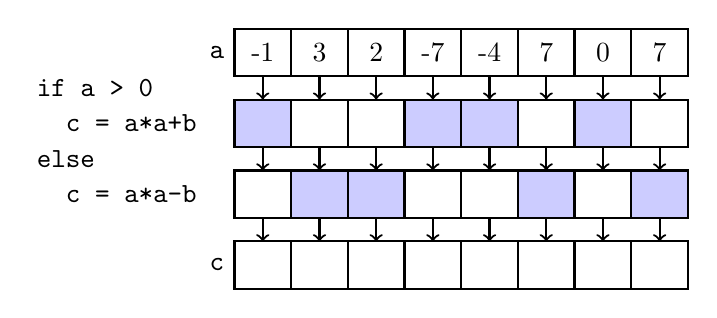
\begin{tikzpicture}[scale=0.6,thick]
    \foreach \x/\num in {0/-1, 1.2/3, 2.4/2, 3.6/-7, 4.8/-4, 6/7, 7.2/0, 8.4/7}
    {
        \draw (\x, 0) node {\num} +(-.6, -.5) rectangle ++(.6, .5);
        \ifnum \num > 0
            \draw (\x, -1.5) +(-.6, -.5) rectangle ++(.6, .5);
            \draw[fill=blue!20] (\x, -3) +(-.6, -.5) rectangle ++(.6, .5);
        \else
            \draw[fill=blue!20] (\x, -1.5) +(-.6, -.5) rectangle ++(.6, .5);
            \draw (\x, -3) +(-.6, -.5) rectangle ++(.6, .5);
        \fi
        \draw (\x, -4.5) +(-.6, -.5) rectangle ++(.6, .5);
        \draw[->] (\x, -0.5) -- (\x, -1);
        \draw[->] (\x, -2) -- (\x, -2.5);
        \draw[->] (\x, -3.5) -- (\x, -4);
    }
    \node[anchor=east] at (-0.6, 0)    {\texttt{a}};
    \node[anchor=west] at (-5, -0.75)  {\texttt{if a > 0}};
    \node[anchor=west] at (-5, -1.5)   {\texttt{~~c = a*a+b}};
    \node[anchor=west] at (-5, -2.25)  {\texttt{else}};
    \node[anchor=west] at (-5, -3)     {\texttt{~~c = a*a-b}};
    \node[anchor=east] at (-0.6, -4.5) {\texttt{c}};
\end{tikzpicture}
\caption{Branch divergence in parallel execution.
    Shaded boxes indicate idle threads. Adapted from~\cite{Hijma2023}.
}\label{fig:branching}
\end{figure}

A workgroup can also have shared memory,
in addition to the global memory buffers that are accessible by all workgroups
of a shader invocation.
Whenever data is shared between threads,
it is important to understand how much synchronization is required,
because the memory model actually makes very few guarantees about the ordering
of memory operations.
Workgroups can be executed with any amount of parallelization and in any order.
Even synchronization within a workgroup is not guaranteed,
but can be enforced with special synchronization barriers.
These barriers have to be passed by all threads of a workgroup simultaneously,
guaranteeing the order of memory operations between threads~\cite{wgsl_spec}.

Many algorithms would however benefit greatly from the ability for
synchroniziation between workgroups.
Newer GPUs do include architectural changes that allow for some amount of
inter-workgroup synchronization~\cite{Hijma2023}.
However this feature is not available in WebGPU due to a limitation within
Metal, which also prohibits using it on other platforms in the spirit of
portability~\cite{Levien2021}.
The topic of synchronization is further discussed in
Section~\ref{subsec:defend_shader} in the context of this work.


\chapter{Implementing the Spectroscopy Algorithm in WebGPU}
\section{Parallelizing the Algorithm}

At the center of this contribution is a parallel GPU-implementation%
\footnote{The code can be found at \url{https://github.com/Gobbel2000/gpuequiv}}
of the energy game introduced in Section~\ref{sec:energy_games}.
Given a game graph as input, it calcu\-lates for each position the energy budgets
required for the attacker, starting at the current position, to win the game.
This algorithm was described in~\cite{bisping2023process} as part of the
spectroscopy algorithm, as well as in~\cite{brihaye2023multi} by T. Brihaye and
A. Goeminne, which more generally covers
\enquote{Multi-Weighted Reachability Games},
but presents essentially the same algorithm structure.

% First, definitions that are also used outside the algorithm
\SetKwData{Updated}{updated}
\SetKwData{Energies}{energies}
\begin{algorithm}[ht]\label{alg:energy_game}
    \DontPrintSemicolon
    \SetKwData{Start}{start}
    \SetKwData{Visit}{visit}
    \SetKwData{New}{new\_energies}
    \SetKwFor{pFor}{for parallel}{do}{end}

    $\Start = \{g \in G_d \mid \mathrm{Succ}(g) = \emptyset\}$\;
    \lFor{$g \in \Start$}{$\Energies[g] = \{\mathbf{0}\}$}
    \lFor{$g \in G \setminus \Start$}{$\Energies[g] = \emptyset$}
    $\Visit = \{\mathrm{Pred}(g) \mid g \in \Start\}$\;

    \BlankLine
    \While{$\Visit \neq \emptyset$}{
        \pFor{$g \in \Visit$}{
            $\Visit = \Visit \setminus \{g\}$\;
            \For{$g' \in \mathrm{Succ}(g)$} {
                $\Updated[g'] = \{ \mathsf{upd}^{-1}(e, w(g, g')) \mid e \in \Energies[g'] \}$
            }

            \BlankLine
            \eIf(\tcp*[h]{attack positions}){$g \in G_a$}{
                $\New = \mathrm{Min} \left(
                    \bigcup_{g' \in \mathrm{Succ}(g)} \uparrow \Updated[g']
                \right)$
            } (\tcp*[h]{defend positions}) {
                $\New = \mathrm{Min} \left(
                    \bigcap_{g' \in \mathrm{Succ}(g)} \uparrow \Updated[g']
                \right)$
            }

            \BlankLine
            \If{$\New \neq \Energies[g]$}{
                $\Energies[g] = \New$\;
                $\Visit = \Visit \cup \mathrm{Pred}(g)$\;
            }
        }
    }
    \Return{\Energies}

    \caption{Parallel Energy Game}
\end{algorithm}

The basic structure is as shown in Algorithm~\ref{alg:energy_game}.
In order to calculate all the winning budgets,
we start at the end of the game graph and work our way backwards.
At all defend positions with no successors the attacker immediately wins,
so we can set the energies required for the attacker to win there to the
0-valued energy tuple (lines 1--3).
In every iteration a set of positions is visited which updates its associated
energies.
The next iteration visits the predecessors of all positions, whose energies
have changed in the previous iteration, thus walking backwards in the game
graph in a breadth-first manner. Once an iteration caused no changes to the
energies, the algorithm terminates.

We achieve parallelization by visiting all positions in the visit list in
parallel, but to fully take advantage of the massively multithreaded
GPU-architecture, each position is further processed by multiple threads.

The core of the algorithm lies in lines 11--15, where the upwards-closed sets of
energies are either unioned or intersected.
Since both operations demand very different approaches,
handling them in a single shader would inevitably incur high branch-divergence.
Therefore both cases are handled by separate, more regular shaders:
one for processing attack positions, another for defend positions.
This technique is known as \enquote{Kernel fission}
and improves resource utilization by allowing threads in a work group to follow
similar instruction paths~\cite{Hijma2023}.
The following two sections detail how these operations have been implemented to
efficiently run on a GPU\@.


\subsection{Attack shader: Union}

In order to calculate the union of the upwards-closed sets,
we can simply unionize the minimal elements that the sets are represented by:

\[\mathrm{Min} \left( \bigcup_{g' \in \mathrm{Succ}(g)} \uparrow \Updated[g'] \right) =
  \mathrm{Min} \left( \bigcup_{g' \in \mathrm{Succ}(g)}          \Updated[g'] \right)\]

The task thus becomes to simply
collect all energies of the current position's successors,
update them accordingly
and then filter out non-minimal energies.
This workflow is sketched out in Figure~\ref{fig:attack}.

\begin{figure}[ht]
\begin{center}
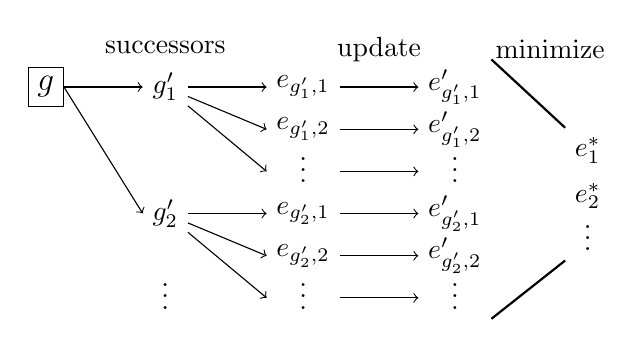
\begin{tikzpicture}
    \node[rectangle,draw] (start_node) {\large{$g$}};
    \node (successor1) [right=of start_node,label=above:successors] {$g_1'$};

    % Energies of successors
    \node (energy1_1) [right=of successor1] {$e_{g_1',1}$};
    \node (energy1_2) [below] at (energy1_1.south) {$e_{g_1',2}$};
    \node (dots1) [below] at (energy1_2.south) {\rvdots};
    \node (energy2_1) [below] at (dots1.south) {$e_{g_2',1}$};
    \node (energy2_2) [below] at (energy2_1.south) {$e_{g_2',2}$};
    \node (dots2) [below] at (energy2_2.south) {\rvdots};

    \node (successor2) [left=of energy2_1] {$g_2'$};
    \node (dots_successors) at (successor2 |- dots2) {\rvdots};

    % Updated energies
    \node (updated1_1) [right=of energy1_1] {$e_{g_1',1}'$};
    \node (updated1_2) [right=of energy1_2] {$e_{g_1',2}'$};
    \node (udots1) at (updated1_2 |- dots1) {\rvdots};
    \node (updated2_1) [right=of energy2_1] {$e_{g_2',1}'$};
    \node (updated2_2) [right=of energy2_2] {$e_{g_2',2}'$};
    \node (udots2) at (updated2_2 |- dots2) {\rvdots};
    % Include energies of g itself
    %\node (energyg_1) [below] at (udots2.south) {$e_{g,1}$};
    %\node (energyg_2) [below] at (energyg_1.south) {$e_{g,2}$};
    %\node (udots3) [below] at (energyg_2.south) {\rvdots};

    % Minimized energies
    \node (minimal1) [right=14mm of udots1.north] {$e_1^*$};
    \node (minimal2) [below] at (minimal1.south) {$e_2^*$};
    \node (mdots) [below] at (minimal2.south) {\rvdots};

    \draw[->] (start_node.east) -- (successor1.west);
    \draw[->] (start_node.east) -- (successor2.west);
    \draw[->] (successor1) -- (energy1_1.west);
    \draw[->] (successor1) -- (energy1_2.west);
    \draw[->] (successor1) -- (energy1_2.west |- dots1);
    \draw[->] (successor2) -- (energy2_1.west);
    \draw[->] (successor2) -- (energy2_2.west);
    \draw[->] (successor2) -- (energy2_2.west |- dots2);

    \draw[->] (energy1_1) -- node (l_update) [above=2mm] {update} (updated1_1);
    \draw[->] (energy1_2) -- (updated1_2);
    \draw[->] (energy1_2.east |- dots1) -- (updated1_2.west |- udots1);
    \draw[->] (energy2_1) -- (updated2_1);
    \draw[->] (energy2_2) -- (updated2_2);
    \draw[->] (energy2_2.east |- dots2) -- (updated2_2.west |- udots2);
    % Energies from g
    %\draw[->,shorten >= 4mm] (start_node.south) |-
    %    node [near end,below] {energies of $g$}
    %    (energyg_2.west);

    % Diagonal lines suggesting the reduction to minimal energies
    \draw[thick] (updated1_1.east |- udots2.south) -- (minimal1.west |- mdots.south);
    \draw[thick] (updated1_1.north east) -- (minimal1.north west);
    \node (l_minimize) [right=7mm of l_update] {minimize};
\end{tikzpicture}
\end{center}
\caption{Data flow for processing Attack positions}%
\label{fig:attack}
\end{figure}

The layout of this figure suggests a very natural way to further parallelize
the processing of attack nodes:
we spawn one thread for each energy tuple.
The shader then has two tasks:
\begin{enumerate}
    \item Update its energy using the correct edge weight,
    \item Figure out if it should be kept as a minimal energy or discarded.
\end{enumerate}

The update step basically follows the definition of $\mathsf{upd}^{-1}$.
Minimizing the energies is done by comparing all energy tuples with each other.
Let $n = \sum_{g' \in \mathrm{Succ}(g)} | \Energies[g'] |$ be the total number
of energies considered for a starting node $g$.
We do $n^2$ comparisons in total, where each thread checks all $n$
energies to find out if this thread's energy is part of the minimal set.
If the thread for energy $e$ encounters an energy $e'$ with $e' \leq e$,
energy $e$ is not minimal and will be filtered out. If $e = e'$, the thread
index is used as a tie breaker to avoid any duplicates.

Theoretically only half of the comparisons could be performed by pruning symmetric
pairs (i.e.\ compare only $e_1$ with $e_2$, not also $e_2$ with $e_1$),
but this would make the comparison itself more expensive by not only requiring
the componentwise comparison of $e_1 \leq e_2$, but also $e_1 \geq e_2$.
Even bigger problems arise when trying to map this approach to the GPU
execution model:
A thread would possibly have to write flags for which energies to keep not only
for its \enquote{own} energy,
but for any energy it's comparing it with.
Such cross-thread memory writes make synchronization more difficult.
Distributing symmetry-reduced comparisons to multiple threads is also
more complex than each thread just comparing its energy with all others.


\subsection{Defend shader: Intersection}

Computing the intersection of upwards-closed sets for processing defend nodes
is significantly more complex than what was done for attack nodes.
The idea behind taking the intersection is that we want to find the set of
energies with which the attacker can win,
regardless of the choice the defender makes.

If $E_1, E_2 \subseteq \mathbf{En}$ are two sets of minimal energies
representing the upwards-closed sets $\uparrow E_1$ and $\uparrow E_2$,
their intersection can be obtained by taking the supremum of all their combinations:
\begin{equation*}
    \mathrm{Min} (\uparrow E_1 \cap \uparrow E_2 ) =
    \mathrm{Min} (\{ \sup(e_1, e_2) \mid e_1 \in E_1,\ e_2 \in E_2 \})
\end{equation*}

In order to handle multiple sets, we iteratively apply that step,
minimizing the result each time.
This approach was proposed in~\cite{brihaye2023multi}.
Line 14 of Algorithm~\ref{alg:energy_game} thus becomes more explicitly:

\begin{algorithm}[ht]\label{alg:intersection}
    \DontPrintSemicolon
    \SetKwData{Intersection}{intersection}
    \SetKwData{New}{new\_energies}

    $\New = \Updated[g_1]$ for some $g_1 \in \mathrm{Succ}(g)$\;
    \For{$g' \in \mathrm{Succ}(g) \setminus \{g_1\}$}{
        $\New = \{\sup(e_1, e_2) \mid e_1 \in \New,\ e_2 \in \Updated[g']\}$\;
        $\New = \mathrm{Min} (\New)$\;
    }

    \caption{Intersection of Upwards-Closed Sets}
\end{algorithm}


\section{Data Layout}

\section{Limitations}


\chapter{Benchmarks and Evaluation of the Implementation}\label{ch:benchmarks}
This chapter will investigate the extent at which GPU-acceleration was able to
speed up execution of the spectroscopy algorithm.
Benchmarks were conducted to compare the performance of the new,
parallelized program \texttt{gpuequiv}
with the original implementation of the same algorithm by Bisping,
created alongside~\cite{bisping2023process}.
We will further look into what was done to verify the correctness of the GPU
implementation.

\section{Benchmarks}

The performance of the implementation was assessed by running it on files from
the \enquote{Very Large Transition System Benchmark Suite} (VLTS)~\cite{vlts},
which, as the name suggests,
includes transition systems with large numbers of states.
For the benchmark, the task is to find the equivalences between \emph{all}
process pairs within a transition system.
The energy game is constructed to include all process pairs that we want to
compare,
but there are some very impactful reductions we can apply to end up with
significantly less than $|\mathsf{Proc}|^2$ starting positions.

Firstly, we can minimize the LTS by consolidating bisimilar processes.
The bisimulation of an LTS can be computed quite efficiently---certainly much
faster than the full spectroscopy algorithm---with the help of a procedure
based around partition refinement~\cite{Blom2002}.
That way we end up with a smaller transition system with just one process for
each bisimulation class of the original system.
Because bisimilarity is already the strongest notion of equivalence,
all processes within a bisimulation class must behave the same for any
equivalence comparison,
so there is no information lost by performing this reduction step.

Secondly,
we can reduce the search space by inspecting the other end of the spectrum.
If two process already aren't enabledness-equivalent,
then none of the other equivalences can hold either,
making any further spectroscopy redundant.
Comparing the enabled actions of two processes is trivially easy,
so any starting positions comparing processes with distinct action sets
can simply be discarded.

The benchmark results are listed in Table~\ref{tab:benchmarks}.
The first column lists the name of the transition system.
Except for \texttt{peterson}, all systems originate from the VLTS Benchmark
Suite.
Next, the number of processes and bisimulation classes ($\sim_B$) is listed,
where $\sim_B$ represents the number of processes left after minimization.
A better metric of the input size for estimating the runtime of the algorithm
is the size of the game graph.
The number of positions and moves is listed.
Finally, the last three columns contain the runtimes of both implementations in
seconds.
The original CPU-based implementation written in the Scala programming
language as part of~\cite{bisping2023process} is listed first,
next to it the runtimes of the GPU-accelerated version \texttt{gpuequiv}.
Both measurements include everything from generating the energy game until
all winning energies are computed, but not the initial minimization step.
The last column lists just the time spent by \texttt{gpuequiv} solving the
energy game, which is where all GPU-computations are situated at.

All benchmarks were run on the same machine with an AMD 5800X processor,
32GB of RAM and an AMD RX 6700XT graphics card with 12GB of VRAM\@.

\begin{table}[htpb]
    \centering
    \caption{Benchmarks for finding all equivalences in an LTS\@.
        The last column shows just the time that \texttt{gpuequiv} spent
        processing the created energy game,
        excluding the time needed to generate the game.
    }%
    \label{tab:benchmarks}
    \small
    \begin{tabular}{@{}l
                    r@{\hskip 6pt}r
                    r@{\hskip 6pt}r
                    S[table-format=3.3]@{\hskip 6pt}
                    S[table-format=2.4]@{\hskip 6pt}
                    S[table-format=1.4]@{}}
        \toprule
        &\multicolumn{2}{c}{LTS size}
        &\multicolumn{2}{c}{Game Graph size}
        &\multicolumn{3}{c}{Runtime (s)} \\
        \cmidrule(lr){2-3} \cmidrule(lr){4-5} \cmidrule(l){6-8}
        LTS~\cite{vlts}
        &$|\mathsf{Proc}|$ &$\sim_B$
        &$|G|$ &$|E|$
        &\cite{bisping2023process} &{gpuequiv} &{Game} \\
        \midrule

        \texttt{peterson}~\cite{bisping2023process}
                              &20     &19     &601        &1856        &0.137 &0.0058 &0.0054 \\
        \texttt{vasy\_0\_1}   &289    &9      &260        &749         &0.018 &0.0046 &0.0044 \\
        \texttt{vasy\_1\_4}   &1183   &28     &520        &1303        &0.019 &0.0052 &0.0050 \\
        \texttt{vasy\_5\_9}   &5486   &145    &1703       &3080        &0.039 &0.0054 &0.0049 \\
        \texttt{vasy\_8\_24}  &8879   &416    &59,531     &145,576     &1.35  &0.066  &0.0417 \\
        \texttt{vasy\_8\_38}  &8921   &219    &7304       &19,634      &0.131 &0.0093 &0.0067 \\
        \texttt{vasy\_10\_56} &10,849 &2112   &1,947,316  &6,044,124   &109.0 &5.46   &4.07   \\
        \texttt{vasy\_18\_73} &18,746 &4087   &75,808,284 &623,482,227 &{--}  &{--}   &{--}   \\
        \texttt{vasy\_25\_25} &25,217 &25,217 &0          &0           &0.217 &0.0078 &0.0021 \\
        \texttt{cwi\_1\_2}    &1952   &1132   &8,503,411  &22,683,038  &229.0 &17.7   &8.91   \\
        \texttt{cwi\_3\_14}   &3996   &62     &11,094     &24,045      &0.192 &0.0227 &0.0193 \\
        \bottomrule
    \end{tabular}
\end{table}

A few notable things can be gathered from the data in
Table~\ref{tab:benchmarks}.
Most importantly, the GPU-accelerated version could in fact achieve
a clear and significant reduction in runtime,
with 10--20x speedups on the larger inputs.
This can mostly be attributed to the high degree of parallelization provided by
the GPU,
but many other factors are also at play.
These benchmarks can not answer the question as to how far one could get with
a purely CPU-based optimized implementation.

Looking at the game graph sizes in relation to the corresponding LTS sizes
gives an impression for how quickly the game graph can explode
and how its size presents the main challenge for any scalable implementation of
the spectroscopy algorithm.
The size of the game is not only dependent on the number of processes in the
input LTS,
but also on its structural properties,
such as how much non-determinism it exhibits
(a process is non-deterministic if it has multiple transitions with the same
action).
This explains why the game graph for \texttt{cwi\_1\_2} is much larger
than the game graph for \texttt{vasy\_10\_56},
even though the latter has almost twice as many states after minimization.
The LTS \texttt{vasy\_25\_25} is a curiosity
because it produces an empty game graph.
This is due to the fact that each processes in this system has a transition
with a unique action,
so there is not a single enabledness-equivalent process pair.
Therefore, there are no starting positions for the game graph and we already
know that no equivalence holds anywhere in the system.

The LTS \texttt{vasy\_18\_73} could not be computed by either implementation
because of memory constraints.
\texttt{gpuequiv} created the energy game in 112 seconds,
but the graph was slightly too large to fit into a GPU buffer:
as mentioned in Section~\ref{subsec:hw_limits},
the largest graph we can load has 536\,870\,911 edges.
Unfortunately that means that,
when looking at this set of benchmarks,
we could not achieve higher scalability by processing larger transition systems
than before.

\section{Correctness}

The correctness of the implementation is verified with an automated test suite.
This includes high-level integration tests checking that the correct
equivalences are reported for an LTS,
as well as more granular unit tests that check individual types or just a
single shader invocation.
A few manually constructed energy games are also tested in addition to the ones
generated by the spectroscopy algorithm
to validate the usability of the library for energy games in general.

Along with the benchmarks, there are some output values included
in~\cite{bisping2023process},
that can be used to verify the results of running the algorithm on the VLTS
files.
This includes the sizes of the equivalence quotients with regards to
enabledness, trace-equivalence and simulation.
These values were reproduced with \texttt{gpuequiv}
and when ensuring that both implementations perform the same operations,
all numbers match up exactly.
This gives a high confidence for the correctness of \texttt{gpuequiv},
even for larger inputs.


\chapter{Conclusion}
The idea of this work was to speed up the algorithm to find all equivalences
within a transition system~\cite{bisping2023process} by running it highly
parallelized on a GPU\@.
This objective was realized by the development of the open source software
library \texttt{gpuequiv}.
It can be used to find all equivalence notions of the
linear-time--branching-time spectrum~\cite{glabbeek1990spectrum}
that equate two or more processes.
This was accomplished with a GPU-accelerated algorithm for processing energy
games that can also be utilized for energy games in general,
not just in the context of the spectroscopy algorithm.
By building on the new WebGPU specification with the implementation of
\texttt{wgpu},
the code can not only run on all major platforms,
but even inside web browsers.

We have shown in Chapter~\ref{ch:implementation} how parallelization could be
applied to the spectroscopy algorithm.
It was found that large parts of work still had to be done on the CPU,
in particular when dealing with the dynamic graph data structures.
For example, generation of the energy game graph had to be done
fully by the CPU for these reasons.
The size of the game graph would have made it an enticing target for
optimization,
but in the end the time spent on generating the game by the CPU does not
outweigh the more complex solving of the resulting energy game.

The most critical parts of solving the energy game could successfully be
computed in parallel on the GPU\@.
This resulted in an overall significant uplift in performance compared to the
previous sequential implementation of~\cite{bisping2023process},
as shown by the benchmarks in Table~\ref{tab:benchmarks}:
The time required to process one particularly large transition system is
reduced from nearly 4 minutes down to just 18 seconds.

Even though care was taken to store data in a highly compressed format
(see~\ref{sec:data}),
the sheer size of the game graph needed to process larger inputs still
ended up exceeding memory limits.
It was therefore not possible to meaningfully increase scalability
over the original implementation.

\subsubsection{Further Work}

While we have focused on the spectrum that was used
in~\cite{bisping2023process},
there is another version of the algorithm that includes many more equivalences
by accounting for silent steps~\cite{bisping2023silent}.
This requires a larger,
more complex game graph and energy values in 8 dimensions instead of 6.
Supporting these additional equivalences would be a way of expanding the
functionality of \texttt{gpuequiv}.
And there is of course always room for further optimization.


\printbibliography[heading=bibintoc]

\end{document}
